\documentclass{article}
% math
\usepackage{amsmath}
\usepackage{bm}
\DeclareMathOperator{\dd}{\mathrm{d}}
% figures
\usepackage{graphicx}
% misc
\usepackage{xcolor} % color text
% refs
\usepackage[style=authoryear,backend=biber]{biblatex}
\addbibresource{refs.bib}
\usepackage{float}
\usepackage{hyperref}
\begin{document}
	\title{Homework Numerical Linear Algebra}
	\author{Arno Strouwen}
	\maketitle
\noindent Only the answers are written here, the questions and the Matlab code to generate the answers can be found \href{https://github.com/arno-training-material/Master-of-Statistics-and-Data-Science/tree/main/Advanced\%20Topics\%20in\%20Data\%20Science}{on my GitHub}.
\\
The zero vector is used as a starting vector $\bm x_0$ for all exercises, that require such a vector.\\
Throughout this document, the size of a square matrix refers to the length of the diagonal of the matrix.
\section*{Exercise 1}
a) $\bm x_1 = \bm x_0 + \bm p_0 = \bm x_0 + A^{-1}\bm r_0 = \bm x_0 + A^{-1}\bm b -A^{-1}A\bm x_0 = A^{-1}\bm b$
\\
b) Proof by induction.
\\
First suppose, $k=0$:
\\
$\bm r_1 = \bm r_0 - A\bm p_0 = \bm r_0 - A(\bm x_1 - \bm x_0) = \bm b - A\bm x_0  -A(\bm x_1 - \bm x_0) = b - A\bm x_1$.
\\
Next, suppose $k$ is any positive integer for which $\bm r_k = b - A\bm x_k$ holds.
Then we have:
\\
$\bm r_{k+1} = \bm r_k - A\bm p_k = \bm b - A\bm x_k- A\bm p_k = \bm b - A\bm x_k - A( \bm x_{k+1} - \bm x_k) = b - A\bm x_{k+1}.$
\\
Where the induction hypothesis is used in the second equality. By the principle of mathematical induction $\bm r_k = b - A\bm x_k$ holds for all positive integers. 
\section*{Exercise 2}
Figure \ref{figex2} shows that the number of iterations required to reach a certain absolute tolerance level behaves linearly in the log-log plot as the size of the tridiagonal matrix $A$ increases. For more stringent tolerances, the number of iterations is shifted upwards. An equation of the form $\log(y) = a\log(x) + b$ is equivalent to $y = e^bx^a$. Here, $a=2$ and $b$ depends on the tolerance. The number of iterations thus increases quadratically as the size of $A$ grows.
\\
\\
Figure \ref{figex2norm} shows that the 2-norm of the residual decreases exponentially as the number of iterations of the algorithm increases.
\begin{figure}
	\centering
	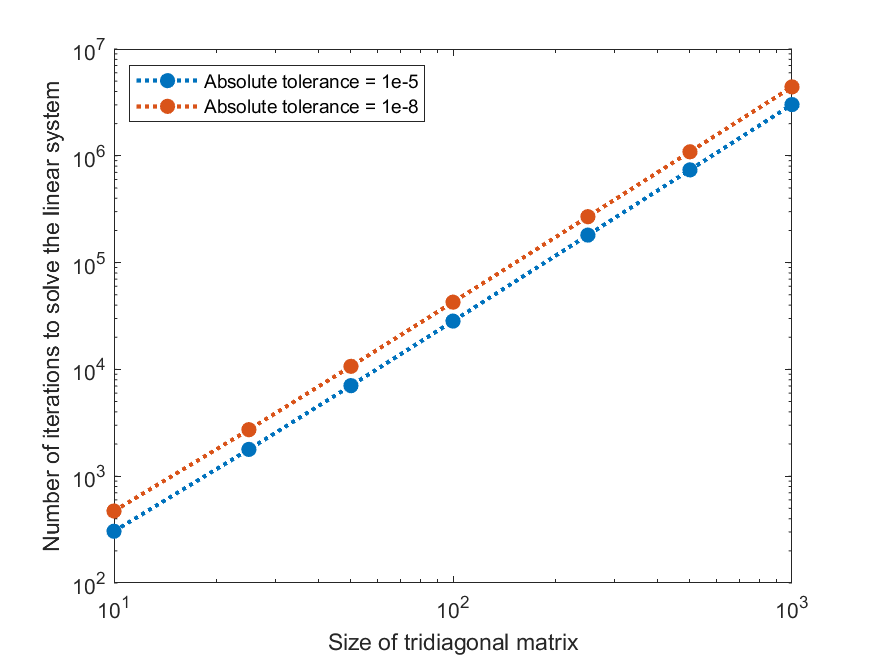
\includegraphics[width=0.8\textwidth]{ex2.png}
	\caption{Quadratic growth of iterations required to solve a sparse linear system using the defect correction algorithm, with $P=2I$.}
	\label{figex2}
\end{figure}
\begin{figure}
	\centering
	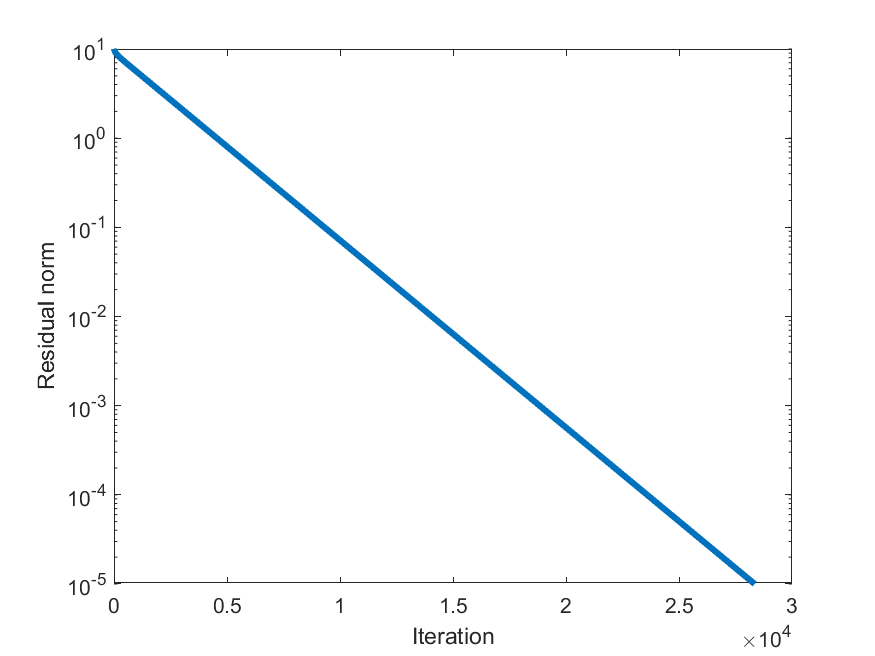
\includegraphics[width=0.8\textwidth]{ex2_norm.png}
	\caption{Exponential decay of residual norm when solving a sparse linear system using the defect correction algorithm, with $P=2I$, where $A$ is a tridiagonal matrix. Size $A = 100$.}
	\label{figex2norm}
\end{figure}
\pagebreak
\section*{Exercise 3}
\textbf{Important:} The equation $A = D - L - U$ makes no sense to me. Clearly $A = D + L + U$ or 
$D = A - L - U$. I'll use my definition for $D$ throughout the remainder of this document. This changes the results for Exercise 4 and 6.
\\
\\
Figure \ref{figex3} shows linear scaling as the Laplace matrix becomes larger (slope is one), in contrast to the quadratic scaling of Figure \ref{figex2}. This is probably why we can solve this system with a matrix of size 10000, while in the previous exercise we stopped at 1000. Exercise 2 also used the Jacobi method (even though the method was not introduced until exercise 3). How is it then possible that we have better scaling here? The behavior of the linear solving thus not only depends on the method, but also on the sparsity pattern of the matrix, which is different between the two exercises.
\\
\\
Figure \ref{figex3norm} still shows exponential decay of the norm of the residual as the number of iterations increases. 
\begin{figure}[H]
	\centering
	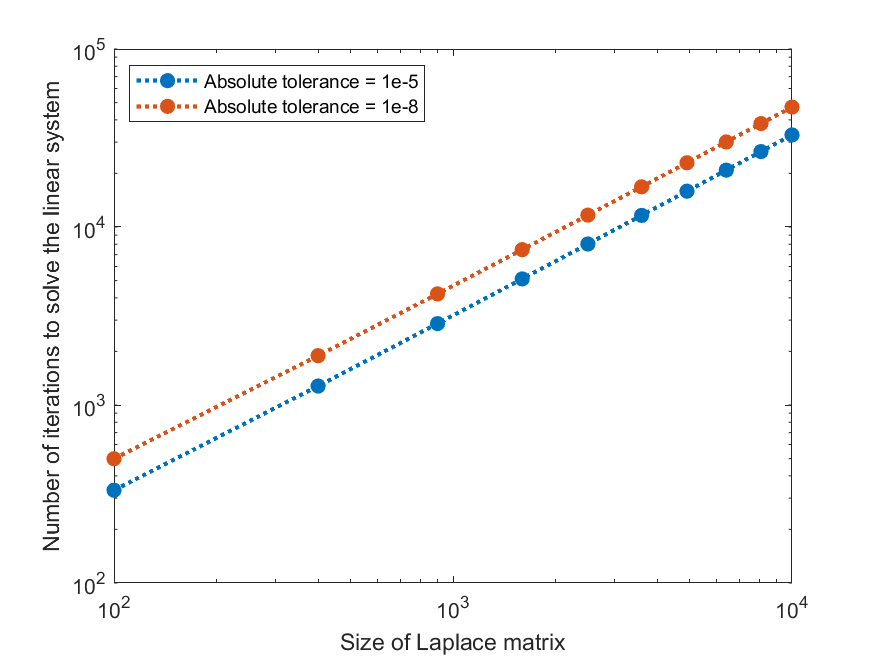
\includegraphics[width=0.8\textwidth]{ex3.png}
	\caption{Linear growth of iterations required to solve a sparse linear system using the Jacobi method,  where $A$ is a Laplace matrix.}
	\label{figex3}
\end{figure}
\section*{Exercise 4}
We use the result from Exercise 1b to prove this:
\\
$D\bm x_{k+1} = D\bm x_k + DP^{-1}\bm r_k =  D\bm x_k + \bm r_k = D\bm x_k + \bm f - A\bm x_k = D\bm x_k + \bm f - (D + L + U)\bm x = -(L+U)\bm x_k + \bm f$.\\
There is an extra minus sign in the solution, compared to the formula in the question.
My solution agrees with the course notes of Professor Vuik on page 21.
\begin{figure}[h]
	\centering
	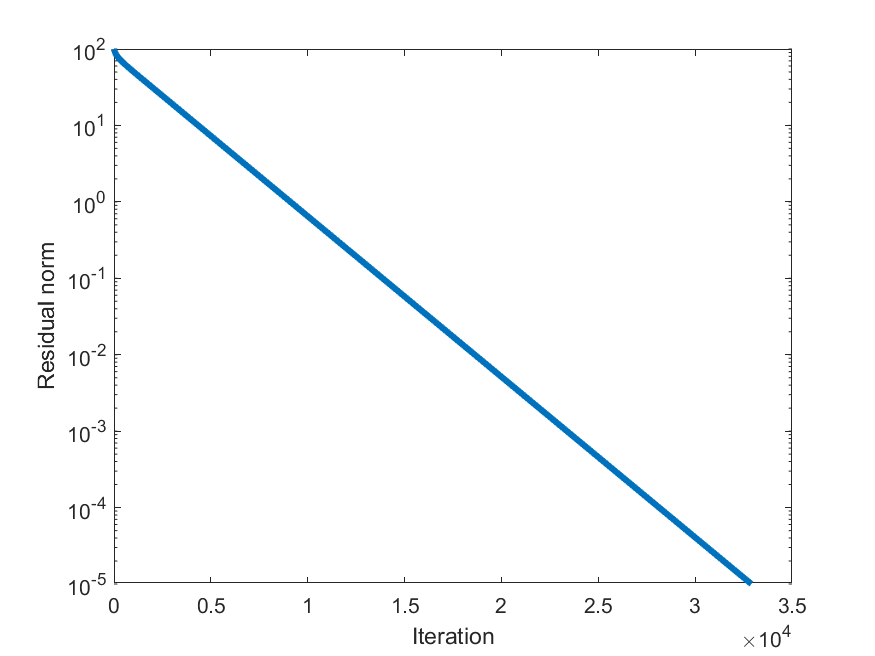
\includegraphics[width=0.8\textwidth]{ex3_norm.png}
	\caption{Exponential decay of residual norm when solving a sparse linear system using the Jacobi method, where $A$ is a Laplace matrix. Size $A = 10000$.}
	\label{figex3norm}
\end{figure}
\section*{Exercise 5}
Figure \ref{figex5} still shows linear scaling as the Laplace matrix becomes larger.
Figure \ref{figex5norm} still shows exponential decay of the norm of the residual as the number of iterations increases. However, by comparing with Figure \ref{figex3}, we see that the Gauss-Seidel methods requires fewer iterations to reach a certain tolerance level.
\section*{Exercise 6}
We use the result from Exercise 1b to prove this:
\\
$(D+L)\bm x_{k+1} = (D+L)\bm x_k + (D+L)P^{-1}\bm r_k =  (D+L)\bm x_k + \bm r_k = (D+L)\bm x_k + \bm f - A\bm x_k = (D+L)\bm x_k + \bm f - (D + L + U)\bm x_k = -U\bm x_k + \bm f$.\\
The minus signs differ, compared to the formula in the question.
My solution agrees with the course notes of Professor Vuik on page 23.
\begin{figure}[H]
	\centering
	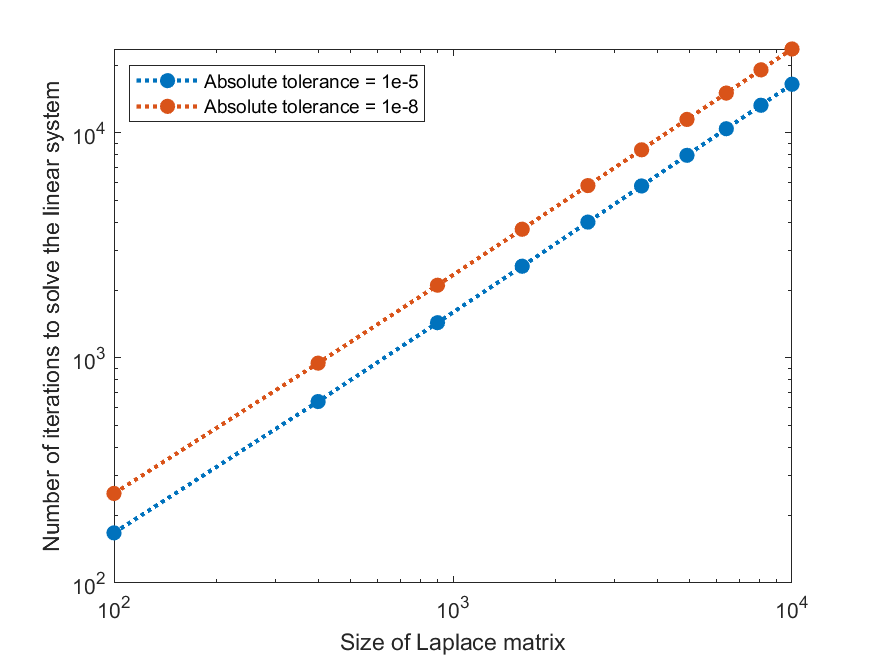
\includegraphics[width=0.8\textwidth]{ex5.png}
	\caption{Linear growth of iterations required to solve a sparse linear system using the Gauss-Seidel method,  where $A$ is a Laplace matrix.}
	\label{figex5}
\end{figure}
\begin{figure}[H]
	\centering
	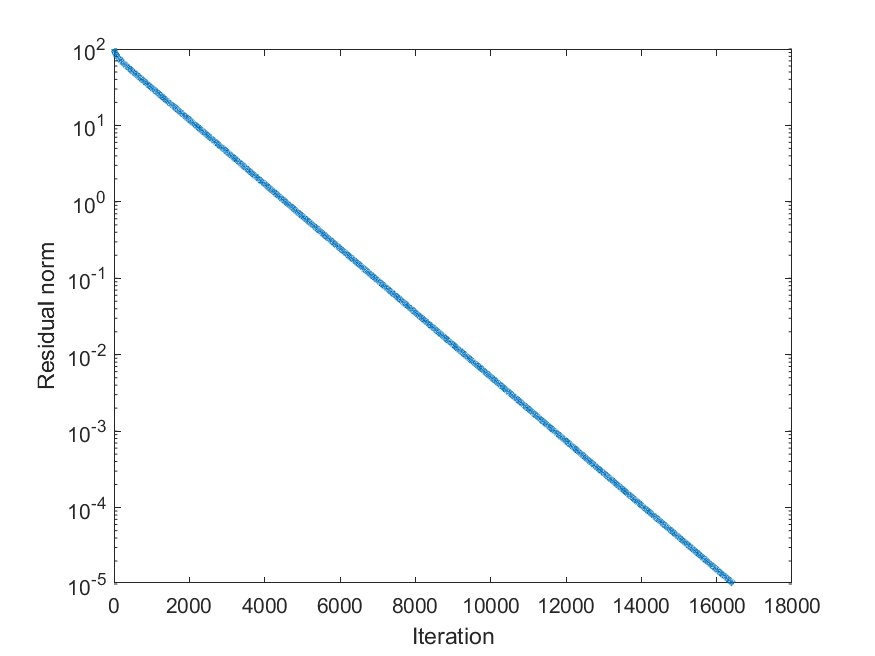
\includegraphics[width=0.8\textwidth]{ex5_norm.png}
	\caption{Exponential decay of residual norm when solving a sparse linear system using the Gauss-Seidel method, where $A$ is a Laplace matrix. Size $A = 10000$.}
	\label{figex5norm}
\end{figure}
\pagebreak
\section*{Exercise 7}
Figure \ref{figex7} still shows linear scaling as the Laplace matrix becomes larger. The number of required iterations for the gradient descent method is very similar to that of the Jacobi method in Figure \ref{figex3}. Figures \ref{figex3norm} and \ref{figex7norm} also show very similar residual norms, except that in the first few iterations of the gradient descent method, the norm of the residual increases. The A-norm of the error also decreases exponentially.
\begin{figure}[H]
	\centering
	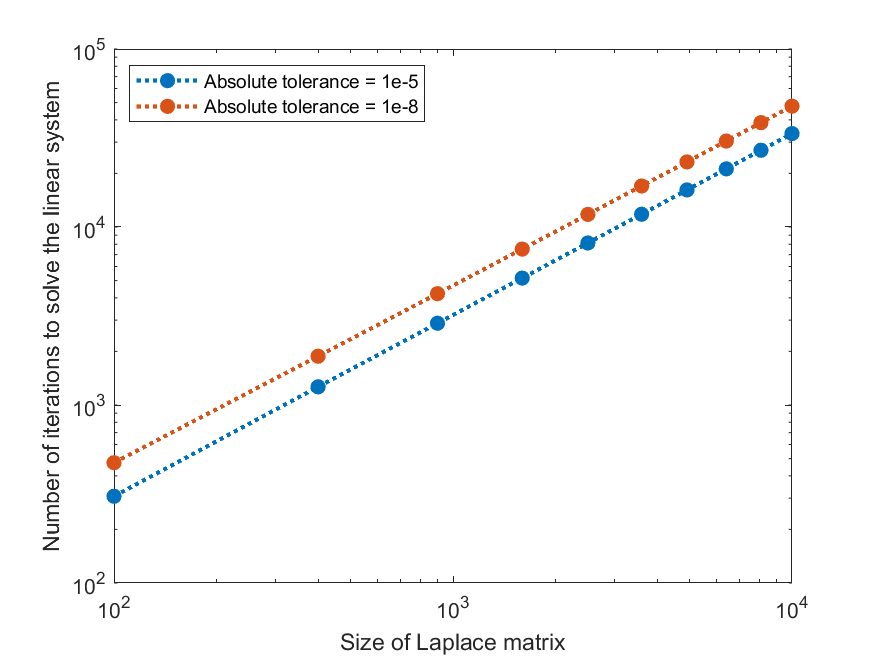
\includegraphics[width=0.8\textwidth]{ex7.png}
	\caption{Linear growth of iterations required to solve a sparse linear system using the gradient descent method,  where $A$ is a Laplace matrix.}
	\label{figex7}
\end{figure}
\begin{figure}[H]
	\centering
	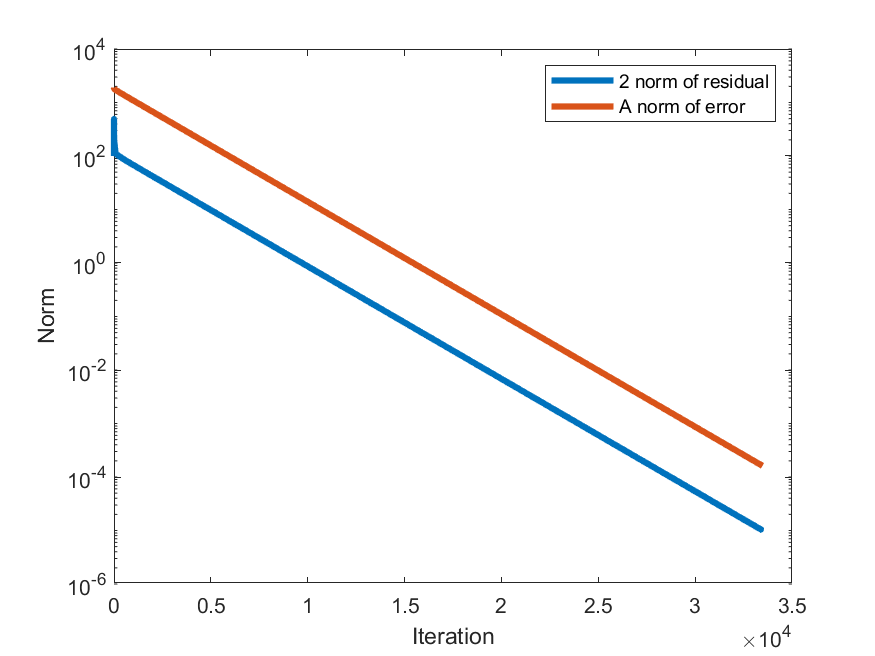
\includegraphics[width=0.8\textwidth]{ex7_norm.png}
	\caption{Exponential decay of residual norm and error norm when solving a sparse linear system using the gradient descent method, where $A$ is a Laplace matrix. Size $A = 10000$.}
	\label{figex7norm}
\end{figure}
\section*{Exercise 8}
Figure \ref{figex8} shows square root scaling as the Laplace matrix becomes larger using the conjugate gradient method (slope equals one half). Figure \ref{figex8norm} shows that the 2 norm of the residuals decreases faster than any of the methods we tried so far. The A-norm of the error also remains under the (pessimistic) theoretical convergence bound for the conjugate gradient method. The linear solver performs much better than the bound at higher iteration counts.
\begin{figure}
	\centering
	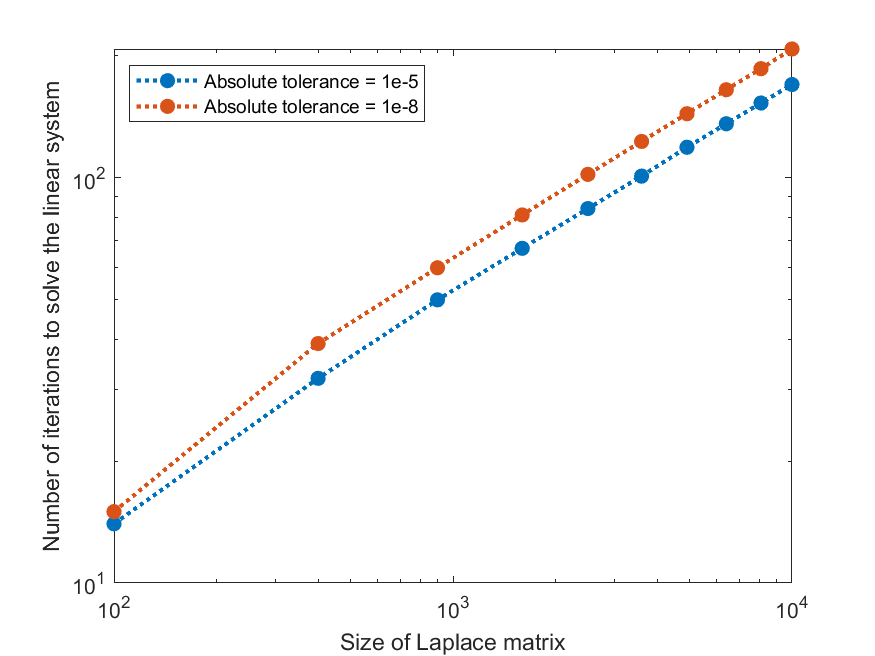
\includegraphics[width=0.8\textwidth]{ex8.png}
	\caption{Square root growth of iterations required to solve a sparse linear system using the conjugate gradient method,  where $A$ is a Laplace matrix.}
	\label{figex8}
\end{figure}
\begin{figure}[h]
	\centering
	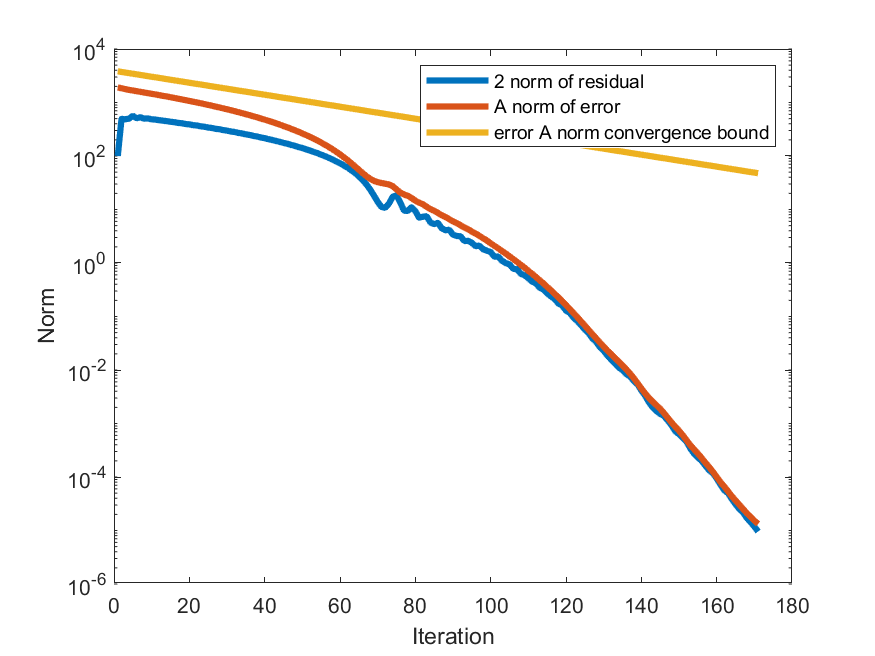
\includegraphics[width=0.8\textwidth]{ex8_norm.png}
	\caption{Fast decay of residual norm and error norm when solving a sparse linear system using the gradient descent method, where $A$ is a Laplace matrix. Size $A = 10000$.}
	\label{figex8norm}
\end{figure}
\section*{Exercise 9}
Little changes when using a diagonal preconditioner for this specific $A$ matrix.
Since this matrix has a constant diagonal, $P=4I$. This means that the condition number of $P^{-1}A$ is the same as the condition number of $A$. The Figures \ref{figex9} and \ref{figex9norm} look almost identical to Figures \ref{figex8} and \ref{figex8norm}, with the preconditioned solver performing slightly better.
\begin{figure}
	\centering
	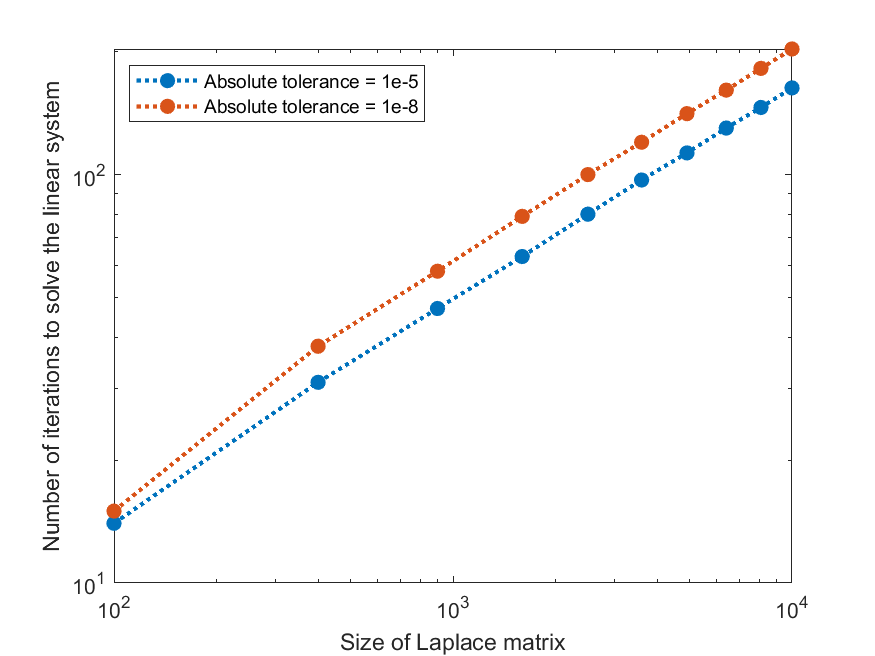
\includegraphics[width=0.8\textwidth]{ex9.png}
	\caption{Square root growth of iterations required to solve a sparse linear system using the preconditioned conjugate gradient method,  where $A$ is a Laplace matrix. Performs slightly better than non-preconditioned solver.}
	\label{figex9}
\end{figure}
\begin{figure}[h]
	\centering
	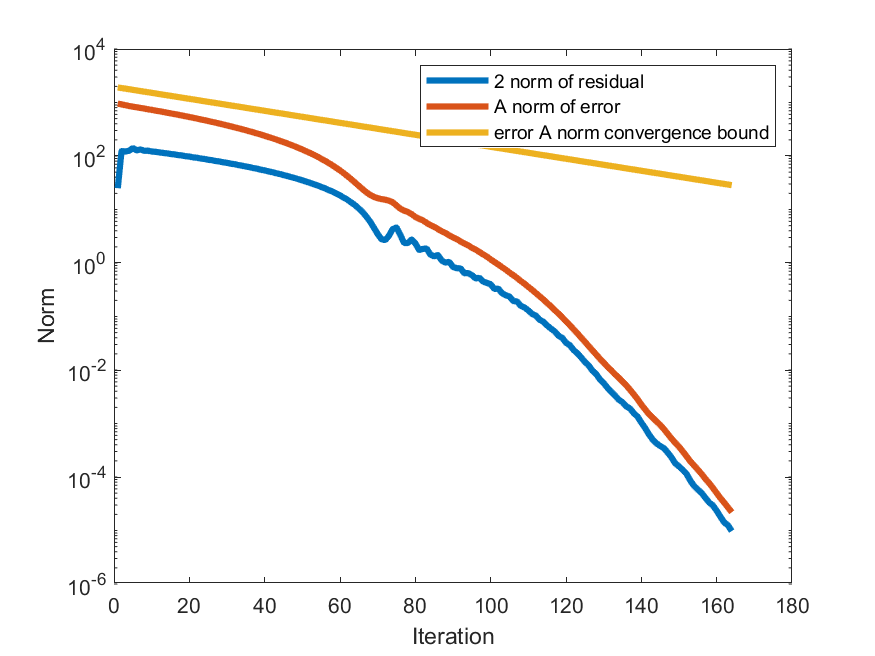
\includegraphics[width=0.8\textwidth]{ex9_norm.png}
	\caption{Fast decay of residual norm and error norm when solving a sparse linear system using the preconditioned gradient descent method, where $A$ is a Laplace matrix. Size $A = 10000$. Performs slightly better than non-preconditioned solver.}
	\label{figex9norm}
\end{figure}
\end{document}